% !TEX root = ../ejemplo-memoria.tex
% Contenidos del capítulo.
% Las secciones presentadas son orientativas y no representan
% necesariamente la organización que debe tener este capítulo.


\section*{Introducción}

En este capítulo se realiza el análisis del sistema desde el punto de vista de la Ingeniería del Software. El objetivo es especificar, de manera estructurada y rigurosa, cómo debe comportarse la aplicación y qué funcionalidades debe ofrecer a los distintos tipos de usuarios, siguiendo las metodologías y herramientas propias de la disciplina.

El análisis comienza con la identificación de los roles principales del sistema y las tareas asociadas a cada uno. En el caso de esta aplicación, los roles contemplados son: usuario registrado, usuario no registrado y administrador. Cada uno de ellos dispone de diferentes permisos y accesos a funcionalidades, siendo el administrador quien puede gestionar todos los contenidos y usuarios, mientras que los usuarios registrados acceden a la experiencia completa de la app.

A continuación, se presentan los diagramas de casos de uso, que permiten visualizar de forma global y por rol las interacciones posibles con el sistema. Posteriormente, se detallan los casos de uso más relevantes mediante tablas descriptivas, especificando actores, propósito, precondiciones, postcondiciones y flujos de eventos. Según la naturaleza de la aplicación, también se incluyen diagramas de actividad y de estados para ilustrar los procesos dinámicos y los posibles cambios de estado de los objetos principales.

\section{Diagramas de casos de uso}

A continuación se presentan los diagramas de casos de uso para los diferentes roles del sistema:



\begin{figure}[H]
    \centering
    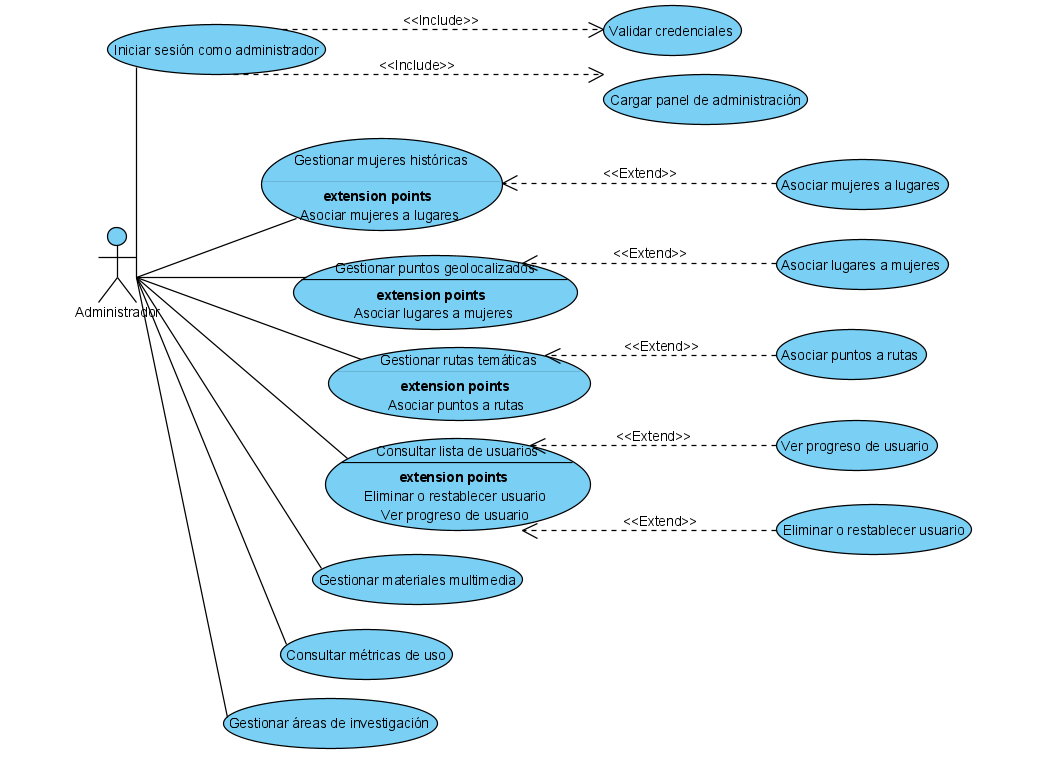
\includegraphics[width=1\textwidth]{figs/diagrama_administrador.png}
    \caption{Diagrama de casos de uso: Administrador}
\end{figure}

\begin{figure}[H]
    \centering
    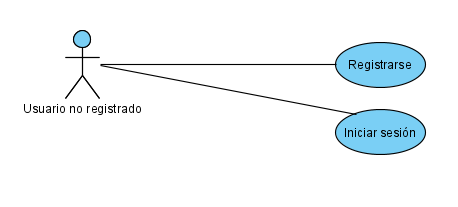
\includegraphics[width=0.8\textwidth]{figs/diagrama_usuario_no_registrado.png}
    \caption{Diagrama de casos de uso: Usuario no registrado}
\end{figure}


\begin{sidewaysfigure}
    \centering
    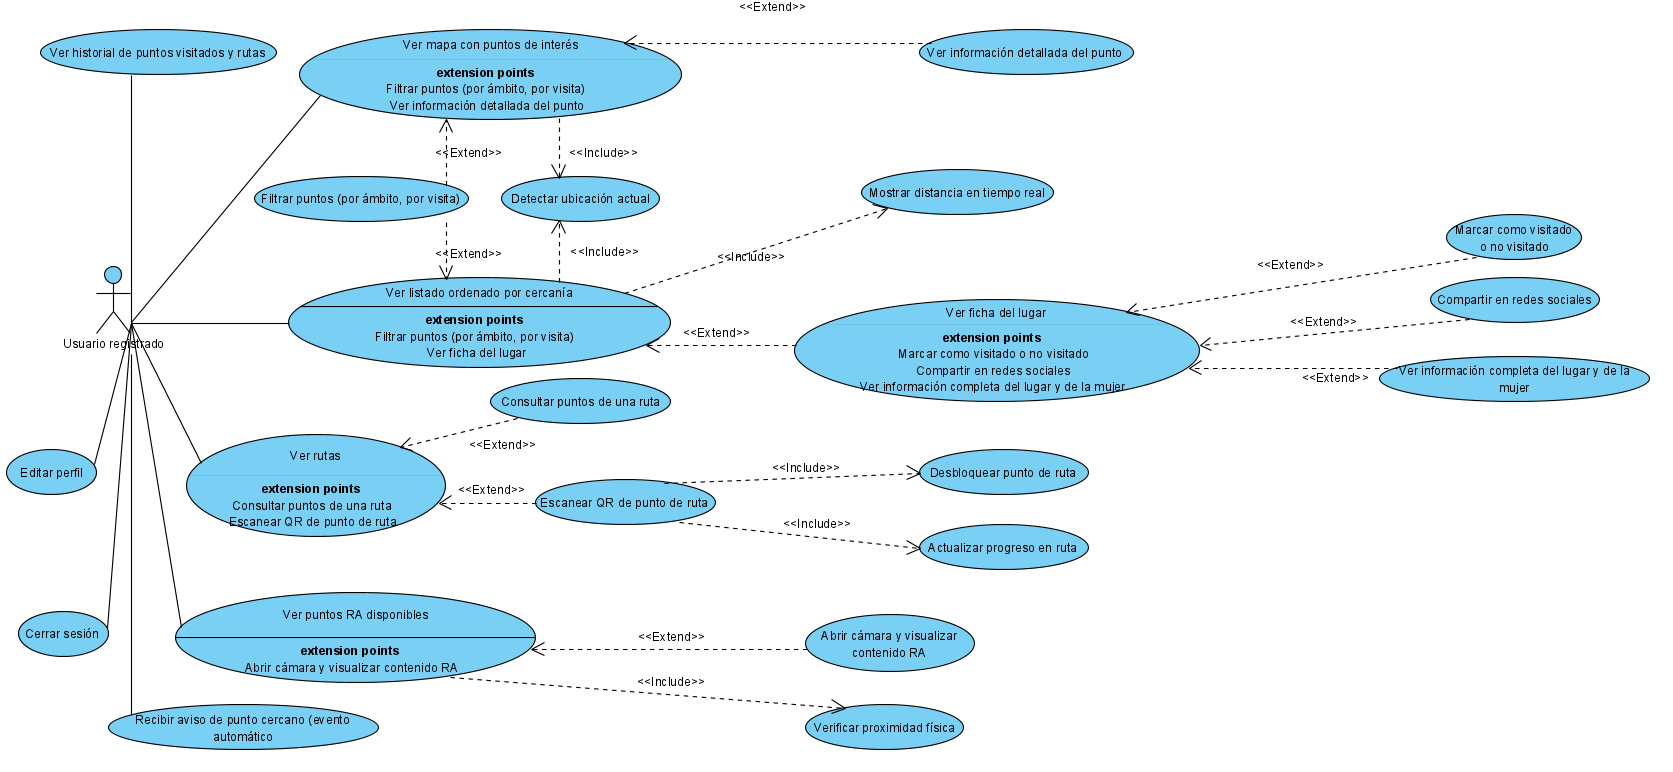
\includegraphics[width=1\textwidth]{figs/diagrama_usuario_registrado.png}
    \caption{Diagrama de casos de uso: Usuario registrado}
\end{sidewaysfigure}


\section{Especificación de casos de uso}

A continuación se detallan los casos de uso principales de la aplicación:
\titlespacing{\subsection}{0pt}{*1}{*0.5} % {izq}{antes}{después}
\subsection{Caso de uso 1: Login de usuario}
\captionsetup{skip=0pt}
\begin{table}[H]
\centering
\caption{Caso de uso 1 - Login de usuario}
\begin{tabular}{|p{4.5cm}|p{10.5cm}|}
\hline
\textbf{Nombre del caso de uso} & Login de usuario \\
\hline
\textbf{Actores} & Usuario no registrado (principal), Sistema (secundario) \\
\hline
\textbf{Propósito} & Permitir que el usuario acceda a su cuenta personal mediante correo electrónico y contraseña. \\
\hline
\textbf{Resumen} & Este caso de uso describe el proceso de inicio de sesión mediante credenciales para acceder a las funcionalidades personalizadas de la app. \\
\hline
\textbf{Tipo} & Primario \\
\hline
\textbf{Referencias} & RF23, RF24, RF25 \\
\hline
\textbf{Precondiciones} & El usuario debe tener una cuenta creada previamente. El sistema debe estar operativo y conectado a internet. \\
\hline
\textbf{Postcondiciones} & El usuario inicia sesión correctamente y accede a la pantalla principal de la aplicación, manteniendo la sesión iniciada hasta que decida cerrarla. \\
\hline
\multicolumn{2}{|c|}{\textbf{Flujo de eventos principal}} \\
\hline
\textbf{Actor} & \textbf{Sistema} \\
\hline
1. El usuario abre la aplicación DONA’m MÓN. & \\
\hline
& 2. El sistema muestra la pantalla de login con los campos de email y contraseña. \\
\hline
3. El usuario introduce su email y contraseña. & \\
\hline
& 4. El sistema valida las credenciales en la base de datos. \\
\hline
& 5. Si las credenciales son válidas, se genera un token y se accede a la pantalla principal. \\
\hline
& 6. Si las credenciales no son válidas, se muestra un mensaje de error y se vuelve al paso 2. \\
\hline
\end{tabular}
\end{table}


\subsection{Caso de uso 2: Registro de usuario}

\begin{table}[H]
\centering
\caption{Caso de uso 2 - Registro de usuario}
\begin{tabular}{|p{4.5cm}|p{10.5cm}|}
\hline
\textbf{Nombre del caso de uso} & Registro de usuario \\
\hline
\textbf{Actores} & Usuario no registrado (principal), Sistema (secundario) \\
\hline
\textbf{Propósito} & Permitir que nuevos usuarios creen una cuenta personal mediante un formulario con correo electrónico y contraseña. \\
\hline
\textbf{Resumen} & Este caso de uso describe el proceso por el cual un usuario puede registrarse en la aplicación, aceptando las condiciones de uso y política de privacidad. \\
\hline
\textbf{Tipo} & Primario \\
\hline
\textbf{Referencias} & RF23, RF24, RF25, RNF21, RNF22 \\
\hline
\textbf{Precondiciones} & El sistema debe estar operativo y conectado. El usuario no debe tener una cuenta registrada con ese correo. \\
\hline
\textbf{Postcondiciones} & El usuario queda registrado y accede automáticamente a la pantalla principal con sesión iniciada. \\
\hline
\multicolumn{2}{|c|}{\textbf{Flujo de eventos principal}} \\
\hline
\textbf{Actor} & \textbf{Sistema} \\
\hline
1. El usuario pulsa sobre "Registrarse" en la pantalla de login. & \\
\hline
& 2. El sistema muestra el formulario de registro con los campos de correo, contraseña y checkbox de aceptación legal. \\
\hline
3. El usuario introduce sus datos y acepta la política de privacidad. & \\
\hline
& 4. El sistema verifica que el correo no exista previamente en la base de datos. \\
\hline
& 5. El sistema guarda los datos cifrados y crea la nueva cuenta. \\
\hline
& 6. El sistema genera una sesión automática y redirige a la pantalla principal. \\
\hline
& 7. Si el correo ya existe o hay errores, se muestra un mensaje al usuario. \\
\hline
\end{tabular}
\end{table}
\subsection{Caso de uso 3: Ver mapa con puntos de interés}

\begin{table}[H]
\centering
\caption{Caso de uso 3 - Ver mapa con puntos de interés}
\begin{tabular}{|p{4.5cm}|p{10.5cm}|}
\hline
\textbf{Nombre del caso de uso} & Ver mapa con puntos de interés \\
\hline
\textbf{Actores} & Usuario registrado (principal), Sistema (secundario) \\
\hline
\textbf{Propósito} & Permitir al usuario visualizar un mapa interactivo con los puntos geolocalizados disponibles en la ciudad de Valencia. \\
\hline
\textbf{Resumen} & Este caso de uso describe la carga del mapa, la detección de la ubicación actual, la visualización de los puntos y la posibilidad de aplicar filtros o acceder a la ficha de un punto. \\
\hline
\textbf{Tipo} & Primario \\
\hline
\textbf{Referencias} & RF1, RF2, RF3, RF7, RF8, RF31, RF32 \\
\hline
\textbf{Precondiciones} & El usuario debe haber iniciado sesión y tener permisos de geolocalización habilitados. \\
\hline
\textbf{Postcondiciones} & El usuario ve los puntos en el mapa y puede filtrar, recibir notificaciones o acceder a la ficha de un punto. \\
\hline
\multicolumn{2}{|c|}{\textbf{Flujo de eventos principal}} \\
\hline
\textbf{Actor} & \textbf{Sistema} \\
\hline
1. El usuario accede a la pestaña del mapa. & \\
\hline
& 2. El sistema obtiene la ubicación actual mediante GPS. \\
\hline
& 3. El sistema carga los puntos geolocalizados en el mapa. \\
\hline
2. El usuario activa un filtro por ámbito o estado de visita. & \\
\hline
& 4. El sistema actualiza la visualización del mapa según los filtros. \\
\hline
3. El usuario pulsa sobre un punto del mapa. & \\
\hline
& 5. El sistema abre la ficha detallada del punto seleccionado. \\
\hline
& 6. Si el usuario se aproxima a un punto no visitado, se lanza una notificación. \\
\hline
\end{tabular}
\end{table}

\subsection{Caso de uso 4: Ver listado de puntos ordenado por cercanía}

\begin{table}[H]
\centering
\caption{Caso de uso 4 - Ver listado de puntos ordenado por cercanía}
\begin{tabular}{|p{4.5cm}|p{10.5cm}|}
\hline
\textbf{Nombre del caso de uso} & Ver listado de puntos ordenado por cercanía \\
\hline
\textbf{Actores} & Usuario registrado (principal), Sistema (secundario) \\
\hline
\textbf{Propósito} & Permitir al usuario consultar todos los puntos disponibles organizados automáticamente por distancia desde su ubicación actual. \\
\hline
\textbf{Resumen} & Este caso de uso permite al usuario visualizar un listado de lugares asociados a mujeres históricas, ordenados por cercanía, con filtros por ámbito y estado, y acceso a la ficha de cada uno. \\
\hline
\textbf{Tipo} & Primario \\
\hline
\textbf{Referencias} & RF7, RF8, RF9, RF31, RF32, RF33, RF34, RF35 \\
\hline
\textbf{Precondiciones} & El usuario debe tener sesión iniciada y el GPS activado. \\
\hline
\textbf{Postcondiciones} & El usuario ve una lista actualizada y filtrada de puntos, con acceso a sus fichas. \\
\hline
\multicolumn{2}{|c|}{\textbf{Flujo de eventos principal}} \\
\hline
\textbf{Actor} & \textbf{Sistema} \\
\hline
1. El usuario accede a la pestaña de listado. & \\
\hline
& 2. El sistema detecta la ubicación actual del usuario. \\
\hline
& 3. El sistema obtiene todos los puntos disponibles. \\
\hline
& 4. El sistema calcula y muestra la distancia en tiempo real a cada punto. \\
\hline
& 5. El sistema ordena el listado por cercanía ascendente. \\
\hline
2. El usuario aplica un filtro por ámbito o por estado de visita. & \\
\hline
& 6. El sistema actualiza el listado aplicando los filtros seleccionados. \\
\hline
3. El usuario pulsa sobre un punto del listado. & \\
\hline
& 7. El sistema abre la ficha detallada del punto. \\
\hline
\end{tabular}
\end{table}

\subsection{Caso de uso 5: Ver ficha del lugar}

\begin{table}[H]
\centering
\caption{Caso de uso 1.5 - Ver ficha del lugar}
\begin{tabular}{|p{4.5cm}|p{10.5cm}|}
\hline
\textbf{Nombre del caso de uso} & Ver ficha del lugar \\
\hline
\textbf{Actores} & Usuario registrado (principal), Sistema (secundario) \\
\hline
\textbf{Propósito} & Permitir al usuario visualizar toda la información del lugar y de la figura femenina representada, incluyendo contenido educativo multimedia. \\
\hline
\textbf{Resumen} & Este caso de uso describe el acceso a la ficha completa de un punto, con texto, imágenes, biografía de la mujer, ubicación y la posibilidad de marcar como visitado o compartir por redes sociales. \\
\hline
\textbf{Tipo} & Primario \\
\hline
\textbf{Referencias} & RF4, RF5, RF12, RF13, RF14, RF36 \\
\hline
\textbf{Precondiciones} & El usuario debe haber accedido desde el mapa o listado, seleccionando un punto. \\
\hline
\textbf{Postcondiciones} & El usuario ha consultado la información y puede haber marcado el punto como visitado o compartido el contenido. \\
\hline
\multicolumn{2}{|c|}{\textbf{Flujo de eventos principal}} \\
\hline
\textbf{Actor} & \textbf{Sistema} \\
\hline
1. El usuario pulsa sobre un punto desde el mapa o el listado. & \\
\hline
& 2. El sistema carga los datos completos del lugar y de la mujer histórica asociada. \\
\hline
& 3. El sistema muestra el contenido educativo (texto, imágenes y/o audio). \\
\hline
2. El usuario pulsa “Marcar como visitado”. & \\
\hline
& 4. El sistema actualiza el estado del punto como visitado y lo guarda en el historial. \\
\hline
3. El usuario pulsa “Compartir”. & \\
\hline
& 5. El sistema lanza el menú para compartir el contenido en redes sociales. \\
\hline
\end{tabular}
\end{table}

\subsection{Caso de uso 6: Ver rutas y consultar puntos de una ruta}

\begin{table}[H]
\centering
\caption{Caso de uso 6 - Ver rutas y consultar puntos de una ruta}
\begin{tabular}{|p{4.5cm}|p{10.5cm}|}
\hline
\textbf{Nombre del caso de uso} & Ver rutas y consultar puntos de una ruta \\
\hline
\textbf{Actores} & Usuario registrado (principal), Sistema (secundario) \\
\hline
\textbf{Propósito} & Permitir al usuario visualizar las rutas temáticas disponibles y consultar qué puntos forman parte de cada una. \\
\hline
\textbf{Resumen} & Este caso de uso describe cómo el usuario accede a la lista de rutas temáticas (por ejemplo, mujeres científicas), y cómo puede consultar los puntos que debe desbloquear escaneando su QR correspondiente. \\
\hline
\textbf{Tipo} & Primario \\
\hline
\textbf{Referencias} & RF11, RF37 \\
\hline
\textbf{Precondiciones} & El usuario debe haber iniciado sesión. \\
\hline
\textbf{Postcondiciones} & El usuario ha accedido a la información de una ruta y conoce qué puntos contiene. \\
\hline
\multicolumn{2}{|c|}{\textbf{Flujo de eventos principal}} \\
\hline
\textbf{Actor} & \textbf{Sistema} \\
\hline
1. El usuario accede a la pestaña de rutas. & \\
\hline
& 2. El sistema muestra una lista de rutas temáticas disponibles, con su nombre y descripción. \\
\hline
2. El usuario pulsa sobre una de las rutas. & \\
\hline
& 3. El sistema muestra los puntos geolocalizados que componen esa ruta. \\
\hline
& 4. El sistema indica visualmente cuáles han sido desbloqueados y cuáles no. \\
\hline
\end{tabular}
\end{table}

\subsection{Caso de uso 7: Escanear QR de punto de ruta}

\begin{table}[H]
\centering
\caption{Caso de uso 7 - Escanear QR de punto de ruta}
\begin{tabular}{|p{4.5cm}|p{10.5cm}|}
\hline
\textbf{Nombre del caso de uso} & Escanear QR de punto de ruta \\
\hline
\textbf{Actores} & Usuario registrado (principal), Sistema (secundario) \\
\hline
\textbf{Propósito} & Permitir al usuario desbloquear un punto dentro de una ruta temática mediante el escaneo de un código QR. \\
\hline
\textbf{Resumen} & Este caso de uso permite que el usuario avance en una ruta únicamente si ha escaneado correctamente el QR asociado a un punto. Una vez validado, se actualiza su progreso. \\
\hline
\textbf{Tipo} & Primario \\
\hline
\textbf{Referencias} & RF30, RF38, RF39 \\
\hline
\textbf{Precondiciones} & El usuario debe haber iniciado sesión y tener la cámara habilitada. Debe haber accedido previamente a la ruta. \\
\hline
\textbf{Postcondiciones} & Si el código escaneado es válido, el punto se marca como desbloqueado en la ruta y se actualiza el historial del usuario. \\
\hline
\multicolumn{2}{|c|}{\textbf{Flujo de eventos principal}} \\
\hline
\textbf{Actor} & \textbf{Sistema} \\
\hline
1. El usuario accede a una ruta y pulsa sobre un punto no desbloqueado. & \\
\hline
2. El usuario pulsa el botón "Escanear QR". & \\
\hline
& 3. El sistema abre la cámara y espera a que el usuario enfoque el código QR. \\
\hline
3. El usuario escanea el QR. & \\
\hline
& 4. El sistema valida que el QR corresponde al punto correcto. \\
\hline
& 5. Si es válido, el sistema desbloquea el punto y lo marca como visitado. \\
\hline
& 6. El sistema actualiza el progreso del usuario en esa ruta. \\
\hline
& 7. Si el código QR no es válido, se muestra un mensaje de error. \\
\hline
\end{tabular}
\end{table}

\subsection{Caso de uso 8: Ver puntos RA disponibles}

\begin{table}[H]
\centering
\caption{Caso de uso 8 - Ver puntos RA disponibles}
\begin{tabular}{|p{4.5cm}|p{10.5cm}|}
\hline
\textbf{Nombre del caso de uso} & Ver puntos RA disponibles \\
\hline
\textbf{Actores} & Usuario registrado (principal), Sistema (secundario) \\
\hline
\textbf{Propósito} & Mostrar al usuario solo los puntos que tienen contenido de realidad aumentada disponible y que están dentro del radio permitido. \\
\hline
\textbf{Resumen} & Este caso de uso describe cómo el sistema filtra automáticamente los puntos que disponen de RA y están dentro del rango de distancia del usuario para que puedan visualizarse. \\
\hline
\textbf{Tipo} & Primario \\
\hline
\textbf{Referencias} & RF40, RF41 \\
\hline
\textbf{Precondiciones} & El usuario debe tener sesión iniciada, el GPS activado y conexión a internet. \\
\hline
\textbf{Postcondiciones} & El usuario visualiza un listado de puntos RA disponibles que puede seleccionar para abrir el contenido RA. \\
\hline
\multicolumn{2}{|c|}{\textbf{Flujo de eventos principal}} \\
\hline
\textbf{Actor} & \textbf{Sistema} \\
\hline
1. El usuario accede a la pestaña de RA. & \\
\hline
& 2. El sistema detecta la ubicación actual del usuario. \\
\hline
& 3. El sistema filtra los puntos con contenido RA. \\
\hline
& 4. El sistema calcula qué puntos RA están dentro del radio permitido. \\
\hline
& 5. El sistema muestra el listado de puntos RA disponibles cercanos. \\
\hline
\end{tabular}
\end{table}

\subsection{Caso de uso 1.9: Visualizar contenido RA}

\begin{table}[H]
\centering
\caption{Caso de uso 9 - Visualizar contenido RA}
\begin{tabular}{|p{4.5cm}|p{10.5cm}|}
\hline
\textbf{Nombre del caso de uso} & Visualizar contenido RA \\
\hline
\textbf{Actores} & Usuario registrado (principal), Sistema (secundario) \\
\hline
\textbf{Propósito} & Permitir al usuario visualizar los modelos 3D o elementos interactivos en RA sobre el entorno real desde la cámara del dispositivo. \\
\hline
\textbf{Resumen} & Este caso de uso describe el proceso de abrir la cámara desde un punto RA cercano y mostrar el contenido de realidad aumentada asociado, como un modelo 3D vinculado a una mujer histórica. \\
\hline
\textbf{Tipo} & Primario \\
\hline
\textbf{Referencias} & RF41 \\
\hline
\textbf{Precondiciones} & El usuario debe haber accedido a la pestaña RA, seleccionado un punto válido y concedido permiso de cámara. \\
\hline
\textbf{Postcondiciones} & El usuario visualiza el contenido RA correctamente alineado sobre el marcador o la ubicación. \\
\hline
\multicolumn{2}{|c|}{\textbf{Flujo de eventos principal}} \\
\hline
\textbf{Actor} & \textbf{Sistema} \\
\hline
1. El usuario pulsa sobre un punto RA disponible. & \\
\hline
& 2. El sistema solicita permisos para acceder a la cámara. \\
\hline
& 3. El sistema abre la cámara del dispositivo. \\
\hline
& 4. El sistema detecta la ubicación o el marcador visual. \\
\hline
& 5. El sistema carga el modelo RA correspondiente (imagen, animación o 3D). \\
\hline
& 6. El sistema muestra el modelo RA en tiempo real superpuesto al entorno. \\
\hline
\end{tabular}
\end{table}

\subsection{Caso de uso 10: Editar perfil de usuario}

\begin{table}[H]
\centering
\caption{Caso de uso 10 - Editar datos del perfil}
\begin{tabular}{|p{4.5cm}|p{10.5cm}|}
\hline
\textbf{Nombre del caso de uso} & Editar datos del perfil \\
\hline
\textbf{Actores} & Usuario registrado (principal), Sistema (secundario) \\
\hline
\textbf{Propósito} & Permitir al usuario modificar sus datos personales como nombre, correo o contraseña desde la sección de perfil. \\
\hline
\textbf{Resumen} & Este caso de uso describe cómo un usuario puede acceder a su perfil, modificar la información personal y guardar los cambios, los cuales se actualizan en la base de datos. \\
\hline
\textbf{Tipo} & Primario \\
\hline
\textbf{Referencias} & RF26, RF42 \\
\hline
\textbf{Precondiciones} & El usuario debe tener sesión iniciada. Debe estar en la sección de perfil. \\
\hline
\textbf{Postcondiciones} & Los datos del perfil del usuario quedan actualizados correctamente en el sistema. \\
\hline
\multicolumn{2}{|c|}{\textbf{Flujo de eventos principal}} \\
\hline
\textbf{Actor} & \textbf{Sistema} \\
\hline
1. El usuario accede a la pestaña de perfil. & \\
\hline
2. El usuario pulsa el botón "Editar perfil". & \\
\hline
3. El usuario modifica los campos deseados. & \\
\hline
4. El usuario pulsa el botón "Guardar cambios". & \\
\hline
& 5. El sistema valida los nuevos datos. \\
\hline
& 6. El sistema actualiza los datos del usuario en la base de datos. \\
\hline
& 7. El sistema muestra un mensaje de confirmación. \\
\hline
\end{tabular}
\end{table}

\subsection{Caso de uso 11: Ver historial de lugares visitados y rutas completadas}

\begin{table}[H]
\centering
\caption{Caso de uso 11 - Ver historial de lugares visitados y rutas completadas}
\begin{tabular}{|p{4.5cm}|p{10.5cm}|}
\hline
\textbf{Nombre del caso de uso} & Ver historial de lugares visitados y rutas completadas \\
\hline
\textbf{Actores} & Usuario registrado (principal), Sistema (secundario) \\
\hline
\textbf{Propósito} & Permitir al usuario consultar qué puntos ha visitado y qué rutas ha completado, con su respectiva fecha y hora. \\
\hline
\textbf{Resumen} & Este caso de uso permite al usuario ver un resumen personalizado de su progreso en la app, incluyendo puntos visitados, rutas completadas y fechas correspondientes. \\
\hline
\textbf{Tipo} & Primario \\
\hline
\textbf{Referencias} & RF14, RF42, F43, F44 \\
\hline
\textbf{Precondiciones} & El usuario debe tener sesión iniciada. \\
\hline
\textbf{Postcondiciones} & El usuario visualiza su historial actualizado, sin modificar ningún dato. \\
\hline
\multicolumn{2}{|c|}{\textbf{Flujo de eventos principal}} \\
\hline
\textbf{Actor} & \textbf{Sistema} \\
\hline
1. El usuario accede a la pestaña de perfil. & \\
\hline
2. El usuario pulsa sobre “Historial de visitas y rutas”. & \\
\hline
& 3. El sistema recupera los datos del historial del usuario desde la base de datos. \\
\hline
& 4. El sistema muestra la lista de puntos visitados con fecha y hora. \\
\hline
& 5. El sistema muestra también las rutas completadas por el usuario. \\
\hline
\end{tabular}
\end{table}


\subsection{Caso de uso 12: Cerrar sesión}

\begin{table}[H]
\centering
\caption{Caso de uso 12 - Cerrar sesión}
\begin{tabular}{|p{4.5cm}|p{10.5cm}|}
\hline
\textbf{Nombre del caso de uso} & Cerrar sesión \\
\hline
\textbf{Actores} & Usuario registrado (principal), Sistema (secundario) \\
\hline
\textbf{Propósito} & Permitir al usuario finalizar su sesión actual y cerrar su acceso a la app hasta el próximo inicio de sesión. \\
\hline
\textbf{Resumen} & Este caso de uso describe cómo el usuario puede cerrar manualmente su sesión desde la sección de perfil, eliminando su token de acceso y volviendo a la pantalla de login. \\
\hline
\textbf{Tipo} & Primario \\
\hline
\textbf{Referencias} & RF25, RF42 \\
\hline
\textbf{Precondiciones} & El usuario debe tener sesión iniciada. \\
\hline
\textbf{Postcondiciones} & La sesión se cierra y el usuario vuelve a la pantalla de login. \\
\hline
\multicolumn{2}{|c|}{\textbf{Flujo de eventos principal}} \\
\hline
\textbf{Actor} & \textbf{Sistema} \\
\hline
1. El usuario accede a la pestaña de perfil. & \\
\hline
2. El usuario pulsa el botón “Cerrar sesión”. & \\
\hline
& 3. El sistema elimina el token de autenticación almacenado. \\
\hline
& 4. El sistema redirige al usuario a la pantalla de login. \\
\hline
\end{tabular}
\end{table}


\subsection{Caso de uso 13: Iniciar sesión como administrador}

\begin{table}[H]
\centering
\caption{Caso de uso 13 - Iniciar sesión como administrador}
\begin{tabular}{|p{4.5cm}|p{10.5cm}|}
\hline
\textbf{Nombre del caso de uso} & Iniciar sesión como administrador \\
\hline
\textbf{Actores} & Administrador (principal), Sistema (secundario) \\
\hline
\textbf{Propósito} & Permitir al administrador acceder al panel de administración web mediante autenticación segura. \\
\hline
\textbf{Resumen} & El administrador introduce sus credenciales (usuario y contraseña) en la pantalla de login del panel de administración. El sistema valida los datos y, si son correctos, permite el acceso a las funcionalidades administrativas. \\
\hline
\textbf{Tipo} & Primario \\
\hline
\textbf{Referencias} & RF16, F20, RNF19 \\
\hline
\textbf{Precondiciones} & El administrador debe estar registrado en el sistema y disponer de credenciales válidas. \\
\hline
\textbf{Postcondiciones} & El administrador accede al panel de administración con los permisos correspondientes. \\
\hline
\multicolumn{2}{|c|}{\textbf{Flujo de eventos principal}} \\
\hline
\textbf{Actor} & \textbf{Sistema} \\
\hline
El administrador accede a la URL del panel de administración. & \\
\hline
El administrador introduce su usuario y contraseña. & \\
\hline
El administrador pulsa el botón de “Iniciar sesión”. & \\
\hline
& 4. El sistema valida las credenciales introducidas. \\
\hline
& 5. Si las credenciales son correctas, el sistema carga el panel de administración. \\
\hline
& 6. Si las credenciales son incorrectas, el sistema muestra un mensaje de error. \\
\hline
\end{tabular}
\end{table}

\subsection{Caso de uso 14: Gestionar mujeres históricas}

\begin{table}[H]
\centering
\caption{Caso de uso 14 - Gestionar mujeres históricas}
\begin{tabular}{|p{4.5cm}|p{10.5cm}|}
\hline
\textbf{Nombre del caso de uso} & Gestionar mujeres históricas \\
\hline
\textbf{Actores} & Administrador (principal), Sistema (secundario) \\
\hline
\textbf{Propósito} & Permitir al administrador crear, editar o eliminar figuras históricas femeninas dentro del sistema. \\
\hline
\textbf{Resumen} & Este caso de uso describe las acciones que puede realizar el administrador para mantener actualizada la base de datos de mujeres históricas: crear nuevas entradas, modificar datos existentes, o eliminarlas. Cada mujer puede estar asociada a uno o varios lugares geolocalizados. \\
\hline
\textbf{Tipo} & Primario \\
\hline
\textbf{Referencias} & RF17, RF18, F21, F22, F24 \\
\hline
\textbf{Precondiciones} & El administrador debe haber iniciado sesión correctamente en el panel de administración. \\
\hline
\textbf{Postcondiciones} & Se actualiza la base de datos de figuras históricas femeninas según las acciones realizadas. \\
\hline
\multicolumn{2}{|c|}{\textbf{Flujo de eventos principal}} \\
\hline
\textbf{Actor} & \textbf{Sistema} \\
\hline
1. El administrador accede a la sección “Mujeres históricas” del panel. & \\
\hline
2. El administrador pulsa sobre “Añadir mujer”, “Editar” o “Eliminar”. & \\
\hline
3. El administrador introduce o modifica datos como nombre, biografía, fechas, y áreas de investigación. & \\
\hline
& 4. El sistema valida los campos requeridos. \\
\hline
& 5. El sistema guarda los datos nuevos o actualizados en la base de datos. \\
\hline
& 6. Si se ha eliminado una figura, se borran también sus asociaciones con puntos. \\
\hline
& 7. El sistema muestra un mensaje de confirmación de los cambios. \\
\hline
\end{tabular}
\end{table}

\subsection{Caso de uso 15: Gestionar puntos geolocalizados}

\begin{table}[H]
\centering
\caption{Caso de uso 15 - Gestionar puntos geolocalizados}
\begin{tabular}{|p{4.5cm}|p{10.5cm}|}
\hline
\textbf{Nombre del caso de uso} & Gestionar puntos geolocalizados \\
\hline
\textbf{Actores} & Administrador (principal), Sistema (secundario) \\
\hline
\textbf{Propósito} & Permitir al administrador crear, editar o eliminar lugares geolocalizados y asociarlos a mujeres históricas. \\
\hline
\textbf{Resumen} & El administrador puede mantener actualizada la base de datos de lugares: crear nuevos puntos, modificar su información (nombre, descripción, ubicación, foto), o eliminarlos. Cada lugar puede estar vinculado a una mujer histórica. \\
\hline
\textbf{Tipo} & Primario \\
\hline
\textbf{Referencias} & RF17, RF18, F22, F24 \\
\hline
\textbf{Precondiciones} & El administrador debe haber iniciado sesión correctamente en el panel de administración. \\
\hline
\textbf{Postcondiciones} & Se actualiza la base de datos de lugares y sus asociaciones con mujeres históricas. \\
\hline
\multicolumn{2}{|c|}{\textbf{Flujo de eventos principal}} \\
\hline
\textbf{Actor} & \textbf{Sistema} \\
\hline
1. El administrador accede a la sección “Lugares” del panel. & \\
\hline
2. El administrador pulsa sobre “Añadir lugar”, “Editar” o “Eliminar”. & \\
\hline
3. El administrador introduce o modifica datos como nombre, descripción, ubicación, foto y mujer asociada. & \\
\hline
& 4. El sistema valida los campos requeridos. \\
\hline
& 5. El sistema guarda los datos nuevos o actualizados en la base de datos. \\
\hline
& 6. Si se elimina un lugar, se eliminan también sus asociaciones. \\
\hline
& 7. El sistema muestra un mensaje de confirmación de los cambios. \\
\hline
\end{tabular}
\end{table}

\subsection{Caso de uso 16: Gestionar rutas temáticas}

\begin{table}[H]
\centering
\caption{Caso de uso 16 - Gestionar rutas temáticas}
\begin{tabular}{|p{4.5cm}|p{10.5cm}|}
\hline
\textbf{Nombre del caso de uso} & Gestionar rutas temáticas \\
\hline
\textbf{Actores} & Administrador (principal), Sistema (secundario) \\
\hline
\textbf{Propósito} & Permitir al administrador crear, editar o eliminar rutas temáticas y asociar puntos a cada ruta. \\
\hline
\textbf{Resumen} & El administrador puede definir rutas temáticas, asignarles nombre y descripción, y asociarles puntos geolocalizados. Puede modificar o eliminar rutas existentes. \\
\hline
\textbf{Tipo} & Primario \\
\hline
\textbf{Referencias} & RF11, RF18b, F24b, F33, F34 \\
\hline
\textbf{Precondiciones} & El administrador debe haber iniciado sesión correctamente en el panel de administración. \\
\hline
\textbf{Postcondiciones} & Se actualiza la base de datos de rutas temáticas y sus asociaciones con puntos. \\
\hline
\multicolumn{2}{|c|}{\textbf{Flujo de eventos principal}} \\
\hline
\textbf{Actor} & \textbf{Sistema} \\
\hline
1. El administrador accede a la sección “Rutas temáticas” del panel. & \\
\hline
2. El administrador pulsa sobre “Añadir ruta”, “Editar” o “Eliminar”. & \\
\hline
3. El administrador introduce o modifica datos como nombre, descripción y puntos asociados. & \\
\hline
& 4. El sistema valida los campos requeridos. \\
\hline
& 5. El sistema guarda los datos nuevos o actualizados en la base de datos. \\
\hline
& 6. Si se elimina una ruta, se eliminan también sus asociaciones. \\
\hline
& 7. El sistema muestra un mensaje de confirmación de los cambios. \\
\hline
\end{tabular}
\end{table}

\subsection{Caso de uso 17: Consultar lista de usuarios}

\begin{table}[H]
\centering
\caption{Caso de uso 17 - Consultar lista de usuarios}
\begin{tabular}{|p{4.5cm}|p{10.5cm}|}
\hline
\textbf{Nombre del caso de uso} & Consultar lista de usuarios \\
\hline
\textbf{Actores} & Administrador (principal), Sistema (secundario) \\
\hline
\textbf{Propósito} & Permitir al administrador visualizar la lista de usuarios registrados, su progreso y gestionar sus cuentas. \\
\hline
\textbf{Resumen} & El administrador puede ver todos los usuarios registrados, consultar su progreso (puntos visitados, logros), y eliminar o restablecer cuentas si es necesario. \\
\hline
\textbf{Tipo} & Primario \\
\hline
\textbf{Referencias} & RF27, RF28, RF29, F25, F26, F27 \\
\hline
\textbf{Precondiciones} & El administrador debe haber iniciado sesión correctamente en el panel de administración. \\
\hline
\textbf{Postcondiciones} & Se actualiza la base de datos de usuarios si se elimina o restablece alguna cuenta. \\
\hline
\multicolumn{2}{|c|}{\textbf{Flujo de eventos principal}} \\
\hline
\textbf{Actor} & \textbf{Sistema} \\
\hline
1. El administrador accede a la sección “Usuarios” del panel. & \\
\hline
2. El administrador selecciona un usuario para ver su perfil y progreso. & \\
\hline
3. El administrador puede eliminar o restablecer la cuenta del usuario. & \\
\hline
& 4. El sistema muestra la información del usuario y su progreso. \\
\hline
& 5. Si se elimina o restablece, el sistema actualiza la base de datos y muestra confirmación. \\
\hline
\end{tabular}
\end{table}

\subsection{Caso de uso 18: Gestionar materiales multimedia}

\begin{table}[H]
\centering
\caption{Caso de uso 18 - Gestionar materiales multimedia}
\begin{tabular}{|p{4.5cm}|p{10.5cm}|}
\hline
\textbf{Nombre del caso de uso} & Gestionar materiales multimedia \\
\hline
\textbf{Actores} & Administrador (principal), Sistema (secundario) \\
\hline
\textbf{Propósito} & Permitir al administrador importar, editar o eliminar imágenes, vídeos y modelos 3D asociados a mujeres o lugares. \\
\hline
\textbf{Resumen} & El administrador puede subir, modificar o eliminar archivos multimedia que se mostrarán en la app, asegurando que el contenido esté actualizado y sea relevante. \\
\hline
\textbf{Tipo} & Primario \\
\hline
\textbf{Referencias} & RF18, F23, F24 \\
\hline
\textbf{Precondiciones} & El administrador debe haber iniciado sesión correctamente en el panel de administración. \\
\hline
\textbf{Postcondiciones} & Se actualiza la base de datos y el repositorio de archivos multimedia. \\
\hline
\multicolumn{2}{|c|}{\textbf{Flujo de eventos principal}} \\
\hline
\textbf{Actor} & \textbf{Sistema} \\
\hline
1. El administrador accede a la sección de gestión multimedia. & \\
\hline
2. El administrador selecciona “Añadir”, “Editar” o “Eliminar” un archivo multimedia. & \\
\hline
3. El administrador sube o modifica el archivo y lo asocia a una mujer o lugar. & \\
\hline
& 4. El sistema valida el formato y tamaño del archivo. \\
\hline
& 5. El sistema guarda o elimina el archivo y actualiza la base de datos. \\
\hline
& 6. El sistema muestra un mensaje de confirmación de los cambios. \\
\hline
\end{tabular}
\end{table}

\subsection{Caso de uso 19: Consultar métricas de uso}

\begin{table}[H]
\centering
\caption{Caso de uso 19 - Consultar métricas de uso}
\begin{tabular}{|p{4.5cm}|p{10.5cm}|}
\hline
\textbf{Nombre del caso de uso} & Consultar métricas de uso \\
\hline
\textbf{Actores} & Administrador (principal), Sistema (secundario) \\
\hline
\textbf{Propósito} & Permitir al administrador visualizar estadísticas y métricas sobre el uso de la aplicación. \\
\hline
\textbf{Resumen} & El administrador puede consultar datos como puntos más visitados, número de usuarios activos, rutas más populares, etc., para tomar decisiones informadas sobre el contenido y la gestión. \\
\hline
\textbf{Tipo} & Primario \\
\hline
\textbf{Referencias} & RF18c, F24c, F28 \\
\hline
\textbf{Precondiciones} & El administrador debe haber iniciado sesión correctamente en el panel de administración. \\
\hline
\textbf{Postcondiciones} & No aplica (consulta de información). \\
\hline
\multicolumn{2}{|c|}{\textbf{Flujo de eventos principal}} \\
\hline
\textbf{Actor} & \textbf{Sistema} \\
\hline
1. El administrador accede a la sección de métricas del panel. & \\
\hline
2. El administrador selecciona el tipo de métrica o informe a consultar. & \\
\hline
& 3. El sistema muestra los datos solicitados en pantalla. \\
\hline
\end{tabular}
\end{table}

\subsection{Caso de uso 20: Gestionar áreas de investigación}

\begin{table}[H]
\centering
\caption{Caso de uso 20 - Gestionar áreas de investigación}
\begin{tabular}{|p{4.5cm}|p{10.5cm}|}
\hline
\textbf{Nombre del caso de uso} & Gestionar áreas de investigación \\
\hline
\textbf{Actores} & Administrador (principal), Sistema (secundario) \\
\hline
\textbf{Propósito} & Permitir al administrador crear, editar o eliminar áreas de investigación asociadas a mujeres históricas. \\
\hline
\textbf{Resumen} & El administrador puede mantener actualizada la lista de áreas de investigación, que luego pueden asociarse a las mujeres históricas para facilitar la búsqueda y filtrado en la app. \\
\hline
\textbf{Tipo} & Primario \\
\hline
\textbf{Referencias} & RF18b, F24b \\
\hline
\textbf{Precondiciones} & El administrador debe haber iniciado sesión correctamente en el panel de administración. \\
\hline
\textbf{Postcondiciones} & Se actualiza la base de datos de áreas de investigación. \\
\hline
\multicolumn{2}{|c|}{\textbf{Flujo de eventos principal}} \\
\hline
\textbf{Actor} & \textbf{Sistema} \\
\hline
1. El administrador accede a la sección de áreas de investigación. & \\
\hline
2. El administrador pulsa sobre “Añadir”, “Editar” o “Eliminar” área. & \\
\hline
3. El administrador introduce o modifica el nombre del área. & \\
\hline
& 4. El sistema valida el campo requerido. \\
\hline
& 5. El sistema guarda o elimina el área en la base de datos. \\
\hline
& 6. El sistema muestra un mensaje de confirmación de los cambios. \\
\hline
\end{tabular}
\end{table}

\section{Diagramas de Actividad}

Los diagramas de actividad son una herramienta utilizada en el modelado de procesos y flujos de trabajo dentro de un sistema. Permiten representar gráficamente la secuencia de actividades, decisiones y flujos alternativos que pueden ocurrir durante la ejecución de un proceso. Son especialmente útiles para visualizar el comportamiento dinámico de un sistema y entender cómo interactúan los distintos componentes o usuarios.

A continuación se muestra un ejemplo de diagrama de actividad correspondiente al flujo de registro e inicio de sesión de usuarios:

\begin{figure}[H]
    \centering
    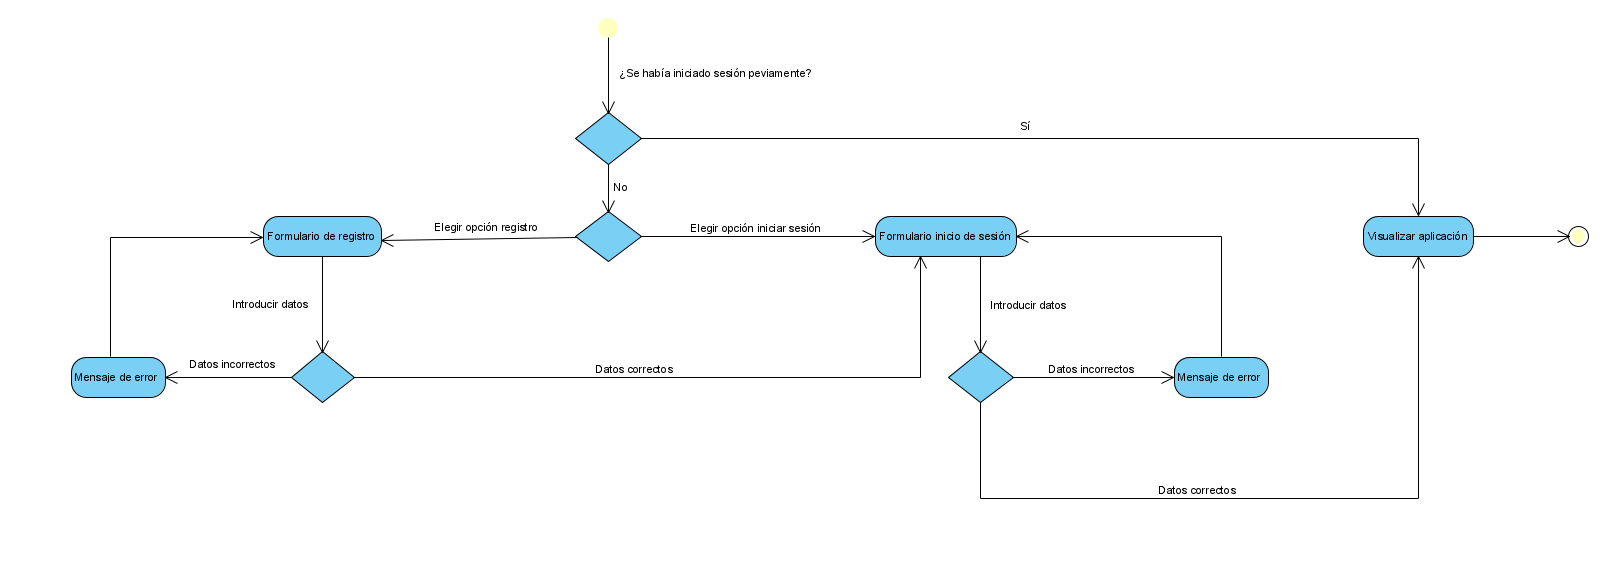
\includegraphics[width=1\textwidth]{figs/diagrama_actividad_usuario_no_registrado.png}
    \caption{Diagrama de actividad de usuario no registrado}
\end{figure}

En este diagrama se observa el proceso que sigue un usuario desde que accede a la aplicación, pasando por las opciones de registro o inicio de sesión, la validación de datos y la visualización de la aplicación, incluyendo el manejo de errores en caso de datos
